\chapter{\label{a3-extractors}Charge Extractor Investigations}

\minitoc

\notes[inline,caption={}]{
	\section{Plan}
	\subsection{Topics}
	\begin{itemize}
		\item RMS extracted charge with varying integration window size and shift with different NSBs and amplitudes (and combination of amplitudes)
		\item Charge resolution of different methods with different NSB (including full integration method)
		\item in the absence of the need for peak finding (laser illumination), and when peak finding is important (Cherenkov) - split into two, best integration technique (different NSBs, different integration window sizes), and best peak finding (different NSBs, need Cherenkov data)
		\item window size might actually change for Cherenkov - got to capture entire signal, and signal might not be centred at "calculated peak time".
	\end{itemize}
	\subsection{Questions}
	\begin{itemize}
		\item ?
	\end{itemize}
}

\section{Introduction}

In Chapter~\ref{ch6-reduction}, the different algorithms for extracting charge from a waveform are extensively discussed, as well as the important considerations one must be vigilant of when producing a charge-extraction algorithm. This purpose of this Appendix is to inform about the performance of the chosen charge-extraction combination, \textit{Cross Correlation} and \textit{Neighbour Peak Finding}, in comparison to typical charge-extraction approaches, in the context of \gls{chec-s}.

\section{Integration Window}

\begin{figure}
  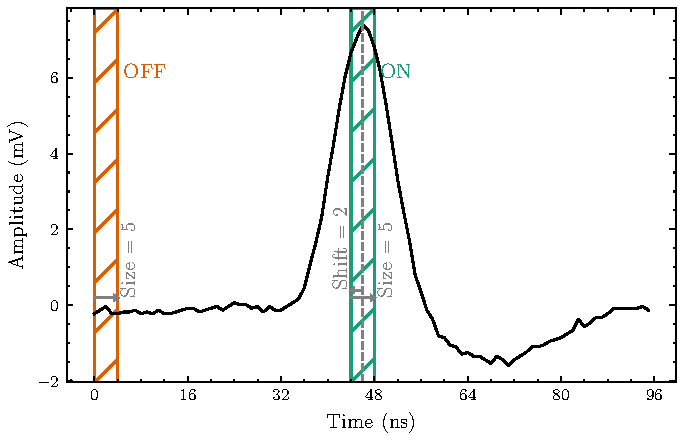
\includegraphics[width=\textwidth]{charge_extraction_window_wf}
  \caption[Definition of integration window on a waveform.]{Example waveform from a Monte Carlo simulation of CHEC-S, containing an approximately \SI{50}{\pe} signal. The ``on'' and ``off'' regions used to extract the signal-to-noise are illustrated. The window start position is defined as the peak position subtracted by the window shift. The window end position is defined as the window start plus the window size. A window size of 5 corresponds to 5 samples being included in the integration.}
  \label{fig:charge_extraction_window_wf}
\end{figure}

\begin{figure}
  \begin{subfigure}[b]{0.49\textwidth}
    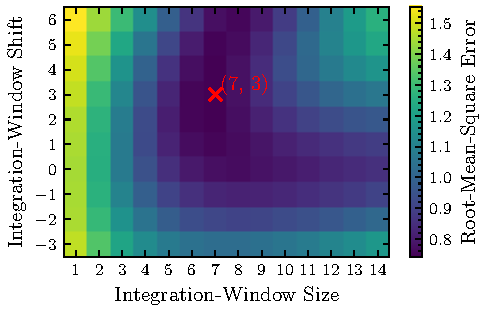
\includegraphics[width=\textwidth]{amp1nsb5}
    \caption{1~p.e. illumination, 5~MHz noise.}
    \label{fig:amp1nsb5}
  \end{subfigure}
  \hfill
  \begin{subfigure}[b]{0.49\textwidth}
    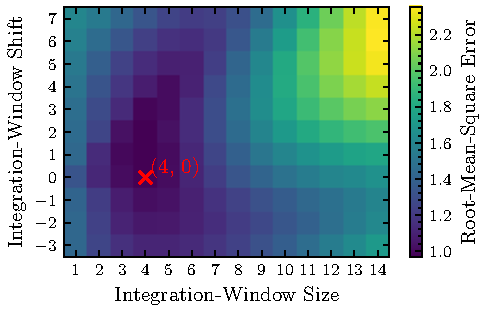
\includegraphics[width=\textwidth]{amp1nsb125}
    \caption{1~p.e. illumination, 125~MHz noise.}
    \label{fig:amp1nsb125}
  \end{subfigure}
  \hfill
  \begin{subfigure}[b]{0.49\textwidth}
    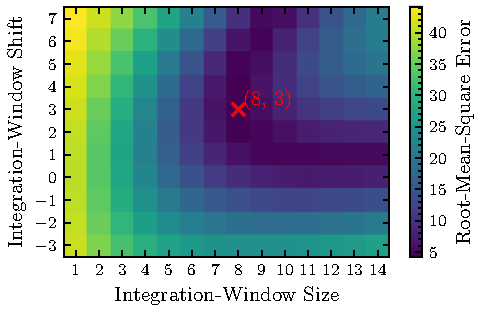
\includegraphics[width=\textwidth]{amp50nsb5}
    \caption{50~p.e. illumination, 5~MHz noise.}
    \label{fig:amp50nsb5}
  \end{subfigure}
  \hfill
  \begin{subfigure}[b]{0.49\textwidth}
    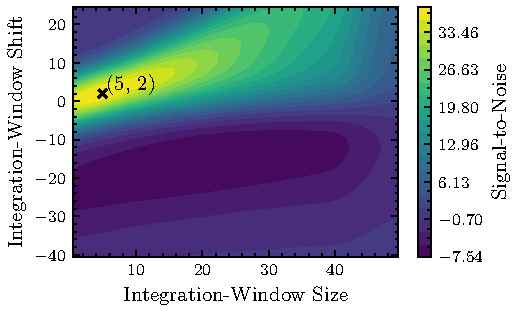
\includegraphics[width=\textwidth]{amp50nsb125}
    \caption{50~p.e. illumination, 125~MHz noise.}
    \label{fig:amp50nsb125}
  \end{subfigure}
  \caption[Optimal integration-window parameters.]{Contour plot of signal-to-noise as a function of window width and shift, for different amplitudes and noise values. The maximum, highlighted with the red annotation, indicates the optimal integration-window parameters when applied to a CHEC-S waveform. The definitions of window and shift are shown in Figure~\ref{charge_extraction_window_wf}. The contours are split into percentiles of the range; the top \SI{5}{\percent} of values are contained in the brightest yellow contour. Negative values correspond to an integration window concentrated on the undershoot of the pulse.}
  \label{fig:snr_noc}
\end{figure}

As an alternative to the \textit{Cross Correlation} integration approach, one may instead use a simple integration window, defined by the number of samples inside the ``window width'', and the number of samples the window is ``shifted'' by from the peak time. In order to investigate the performance of the integration-window approach fairly, one must first optimise the values for the width and shift of the window when extracting charge from a \gls{chec-s} waveform. This exercise was performed using a Monte Carlo simulation of the lab set-up, where the camera was uniformly illuminated. The pulse time is consistent in simulations of this nature, therefore the same pulse time is manually chosen for every waveform. This allows the following investigation to be solely on the integration approach, avoiding the interference from peak finding.

\subsection{Optimal Integration Window Parameters}

As explained in Chapter~\ref{ch6-reduction}, the optimal integration window parameters are noise dependant; a larger integration window is likely to include more noise (\gls{nsb} and \gls{dcr}). However, a larger window size results in more of the signal being captured. In Figure~\ref{fig:snr_noc} the signal-to-noise ($\text{SNR}$) as a function of integration-window parameters is shown for different amplitude and noise values. The $\text{SNR}$ investigation was performed as follows. Assume an ``on'' region of the waveform, where the extracted value contains the signal plus the noise, and an ``off'' region where the extracted value contains solely the noise contributions (Figure~\ref{fig:charge_extraction_window_wf}). The optimal window for a constant signal on top of a fluctuating background is then found by:
\begin{equation}
\text{SNR} = \frac{\mu_\text{on}}{\sigma_\text{off}},
\end{equation}
where $\mu_\text{on}$ is the average signal extracted from the ``on'' region, and $\sigma_\text{off}$ is the standard deviation of the signal extracted from the ``off'' region. This is an alternative to looking for the optimal window for a fluctuating signal on top of a fluctuating background ($\text{SNR} = \frac{\mu_\text{on}}{\sigma_\text{on}}$), which, due to the inclusion of the signal deviations from the ``on'' region, is much less sensitive to the noise fluctuations and has a strong dependence on the signal level, i.e. the Poisson fluctuations of the signal increases with amplitude.

In Figure~\ref{fig:snr_noc} the conflict between a large window size to contain the full signal, and a small window to minimise noise is evident, resulting in a limited region in which a high signal-to-noise can be achieved. In conclusion, an integration window width of 5 samples and a shift of 2 samples appeared to be optimal for a noise of \SI{125}{MHz}, for both small and large amplitudes (Figures~\ref{fig:amp1nsb125} and \ref{fig:amp50nsb125} respectively). This integration window is demonstrated in Figure~\ref{fig:charge_extraction_window_wf}. As the charge resolution requirements are defined at an \gls{nsb} of \SI{125}{MHz}, these window parameters are adopted for the following investigations.

\subsection{Comparison with Cross Correlation}

\begin{figure}
  %\includegraphics[width=\textwidth]{}
  \caption[Charge resolution comparison between Cross Correlation and Window Integration for lab data.]{Charge resolution of the \textit{Cross Correlation} charge extraction approach applied to uniformly illuminated lab data, compared to the charge resolution of the integration window approach for the same dataset.}
  \label{fig:cr_ce_lab}
\end{figure}

\begin{figure}
  %\includegraphics[width=\textwidth]{}
  \caption[Charge resolution comparison between Cross Correlation and Window Integration for MC-lab data with an optical crosstalk of \SI{40}{\percent}.]{Charge resolution of the \textit{Cross Correlation} charge extraction approach compared to the charge resolution of the integration window approach, for both \SI{5}{MHz} and \SI{125}{MHz} \gls{nsb} noise. The dataset contains waveforms obtained from Monte Carlo simulations of the camera uniformly illuminated, replicating the lab set-up. The optical crosstalk of the photosensors in the simulation is \SI{40}{\percent}.}
  \label{fig:cr_ce_mclab_opct40}
\end{figure}

\begin{figure}
  %\includegraphics[width=\textwidth]{}
  \caption[Charge resolution comparison between Cross Correlation and Window Integration for MC-lab data with an optical crosstalk of \SI{20}{\percent}.]{Same as Figure~\ref{fig:cr_ce_mclab_opct40}, but with an optical crosstalk of \SI{20}{\percent}.}
  \label{fig:cr_ce_mclab_opct20}
\end{figure}

\begin{figure}
  %\includegraphics[width=\textwidth]{}
  \caption[Charge resolution comparison between Cross Correlation and Window Integration for MC-lab data with a high amount of electronic noise.]{Same as Figure~\ref{fig:cr_ce_mclab_opct40}, but with a factor of 10 higher electronic noise.}
  \label{fig:cr_ce_mclab_opct20}
\end{figure}

In order to evaluate the performance of the \textit{Cross Correlation} technique with respect to a simple integration window, I calculated the charge resolution for each approach using identical datasets. When applied to our lab dynamic range data, which is obtained in the presence of only dark count noise (estimated to be about \SI{5}{MHz}, there is very little difference between the charge extraction methods.

\change[inline]{robust with NSB}

\change[inline]{Same discriminator used for different NSB}



